% This text is proprietary.
% It's a part of presentation made by myself.
% It may not used commercial.
% The noncommercial use such as private and study is free
% Sep. 2005 
% Author: Sascha Frank 
% University Freiburg 
% www.informatik.uni-freiburg.de/~frank/


\documentclass[aspectratio=169]{beamer}


%%% HANDOUT START
%  \documentclass[11pt,handout,aspectratio=169]{beamer}
%  \usepackage{pgfpages}
%  \pgfpagesuselayout{6 on 1}[a4paper]
%  \setbeamertemplate{footline}{% set footline options
%   $\qquad\qquad$\insertpagenumber   
%   }

 
%%% HANDOUT END

\usefonttheme{professionalfonts}
 
%\setbeamertemplate{page number in head/foot}[totalframenumber]
%\beamertemplatenavigationsymbolsempty

%\setbeamerfont{page number in head/foot}{size=\footnotesize}


%pdfnup --a4paper --keepinfo --nup 1x3 --frame true   --scale 0.92 --no-landscape --outfile handout.pdf slides.pdf


\setbeamercovered{transparent=10}


\usepackage{multirow}
% \usepackage{pgfpages}
% \mode<handout>{\setbeamercolor{background canvas}{bg=black!5}}
% \pgfpagesuselayout{4 on 1}[letterpaper,border shrink=2mm]

%\documentclass[handout]{beamer}
% \setbeamertemplate{bibliography entry title}{}
% \setbeamertemplate{bibliography entry location}{}
% \setbeamertemplate{bibliography entry note}{}
\setbeamertemplate{bibliography item}{\insertbiblabel}

\newcommand{\Prob}{{\rm I\hspace{-0.8mm}P}}

\newcommand{\p}[0]{\mathbf{p}}
\newcommand{\q}[0]{\mathbf{q}}

\newcommand{\e}[0]{\textbf{e}}
\newcommand{\PP}[0]{\mathbf{P}}
\newcommand{\II}[0]{\textbf{I}}
\newcommand{\Q}[0]{\mathbf{Q}}
\newcommand{\E}[0]{\mathbb{E}}
\newcommand{\X}[0]{\textbf{X}}
\newcommand{\Z}[0]{\textbf{Z}}
\newcommand{\s}[0]{\mathbf{s}}
\newcommand{\C}[0]{\textbf{C}}
\newcommand{\es}[0]{\mathbf{s}}
\newcommand{\trev}[0]{\overleftarrow}
\definecolor{mygray}{gray}{0.6}
\newcommand{\diag}{\mathbf{diag}}
\newcommand{\iii}[0]{\mathbf{i}}

%\dual to oznacznie dualnosci, oryginalnie *
%\newcommand{\dual}[0]{\circledast}
\newcommand{\dual}[0]{*}

%\monD to oznacznie tej drugiej monotonicznosci, czyli np. ^\monD-Mobius monotonicity
%\newcommand{\monD}[0]{\lozenge}
\newcommand{\monD}[0]{\downarrow}
\newcommand{\monU}[0]{\uparrow}

\usepackage{cancel} 

\usepackage{dsfont}
 
\newcommand{\indic}[0]{\mathds{1}}
\usepackage{pdfpages}
\usepackage{graphicx}
\usepackage{soul} 
\usepackage{tikz}
\usepackage[utf8]{inputenc}
\usepackage[T1]{fontenc}
\usetikzlibrary{arrows}




\setbeamertemplate{theorems}[numbered]

% Add support for \subsubsectionpage
%\def\subsubsectionname{\translate{Subsubsection}}
%\def\insertsubsubsectionnumber{\arabic{subsubsection}}
% \setbeamertemplate{subsubsection page}
% {
%   \begin{centering}
%     {\usebeamerfont{subsubsection name}\usebeamercolor[fg]{subsubsection name}\subsubsectionname~\insertsubsubsectionnumber}
%     \vskip1em\par
% %     \begin{beamercolorbox}[sep=4pt,center]{d part title}
% %       \usebeamerfont{subsubsection title}\insertsubsubsection\par
% %     \end{beamercolorbox}
%   \end{centering}
% }
% \def\subsubsectionpage{\usebeamertemplate*{subsubsection page}}


\AtBeginSection{\frame{\sectionpage}}
\AtBeginSubsection{\frame{\subsectionpage}}
\AtBeginSubsubsection{\frame{\subsubsectionpage}}
 
\usepackage{tikz}

\usepackage{pgfplots}
\pgfplotsset{compat=1.11}
 

 % FROM BOOK:
 


\usepackage{algorithm}

\usepackage{algpseudocode}
\usepackage{caption}
\usepackage{comment}
\usepackage{booktabs}


 \usepackage[T1]{fontenc}
%\usepackage[utf8]{inputenc}
%\usepackage[polish]{babel}

\usepackage{tikz}
\usetikzlibrary{arrows}
\usetikzlibrary{arrows.meta}
\usetikzlibrary{patterns}
%\usetikzlibrary{decorations.pathreplacing,calligraphy}
\usetikzlibrary{decorations.text}
\usetikzlibrary{decorations.markings}
\usetikzlibrary{decorations.pathreplacing}
\usetikzlibrary{arrows.meta,babel}
\usetikzlibrary{shapes.misc}

\usepackage{pgfplots}
%\pgfplotsset{compat=1.7}
\pgfplotsset{compat=1.16}
%\pgfplotsset{compat=1.18}
\usepgfplotslibrary{fillbetween}

\usepackage{subfig}

\usepackage{etoolbox}


% 2. Configuration Commands
% ============================
% Code listings (for \begin{lstlisting}...\end{lstlisting})
\usepackage{listings}
\lstset{
  basicstyle=\ttfamily\footnotesize,
  columns=fullflexible,
  keepspaces=true,
  showstringspaces=false,
  frame=none,
  numbers=none,
  breaklines=true,
}
%
% \renewcommand{\lstlistingname}{Python Listing} % Listing -> Algorithm
% \lstset{basicstyle=\fontsize{8}{12}\selectfont\ttfamily}
% \lstset{language=Python}
%
% \captionsetup[figure]{font=small} % Changes font size in figure captions
%
% \captionsetup[algorithm]{font=normal} % Changes font size in algorithm captions
% \AtBeginEnvironment{algorithmic}{\normalsize} % Changes font size inside algorithm body
%


% --- Bold (\bf) Commands ---


\newcommand{\bfM}{\mathbf{M}}
\newcommand{\bfU}{\mbox{\boldmath $U$}}
\newcommand{\bfu}{\mbox{\boldmath$u$}}
\newcommand{\bfv}{\mathbf{v}}
\newcommand{\bfw}{\mathbf{w}}
\newcommand{\bfx}{\mathbf{x}}
\newcommand{\done}{\textbf{\textcolor{red}{DONE }}}
\newcommand{\bfy}{\mbox{\boldmath$y$}}
\newcommand{\bfz}{\mathbf{z}}
\newcommand{\bfg}{\mbox{\boldmath$g$}}
\newcommand{\bfh}{\mbox{\boldmath$h$}}
\newcommand{\bfb}{\mbox{\boldmath$b$}}
\newcommand{\bfp}{\mathbf{p}}
\newcommand{\bfq}{\mathbf{q}}
\newcommand{\bfJ}{\mbox{\boldmath $J$}}
\newcommand{\bfP}{\mathbf{P}}
%\newcommand{\bfT}{\mbox{\boldmath $T$}}
\newcommand{\bfT}{\vec{T}}
\newcommand{\bfL}{\mathbf{L}}
\newcommand{\bfm}{\mbox{\boldmath$m$}}

\newcommand{\bfSigma}{\boldsymbol{\Sigma}}
\newcommand{\bfsigma}{\mbox{\boldmath $\sigma$}}
\newcommand{\bfmu}{\mbox{\boldmath $\mu$}}
\newcommand{\bfzero}{{\bf 0}}


\newcommand{\bfa}{\boldsymbol{a}}
\newcommand{\bfA}{\mathbf{A}}
\newcommand{\bfB}{\mathbf{B}}
\newcommand{\bbX}{\mathbb{X}}
\newcommand{\bfX}{\mathbf{X}}
\newcommand{\bfY}{\mathbf{Y}}
\newcommand{\bfZ}{\mathbf{Z}}
\newcommand{\bfV}{\mbox{\boldmath $V$}}
\newcommand{\bfC}{\mathbf{C}}
\newcommand{\bbR}{\mathbb{R}}
\newcommand{\bbN}{\mathbb{N}}
\newcommand{\bbZ}{\mathbb{Z}}
\newcommand{\bfS}{\mathbf{S}}
\newcommand{\bfD}{\mathbf{D}}
\newcommand{\bff}{\mathbf{f}}
\newcommand{\bfF}{\mathbf{F}}
\newcommand{\bfI}{\mathbf{I}}
\newcommand{\bfe}{\mathbf{e}}
\newcommand{\bfk}{\mbox{\boldmath$k$}}
\newcommand{\bfn}{\mbox{\boldmath$n$}}
\newcommand{\bfR}{\mathbf{R}}
\newcommand{\bfQ}{\mathbf{Q}}
\newcommand{\bfG}{\mbox{\boldmath $G$}}

\newcommand{\bfPi}{\mbox{\boldmath $\Pi$}}
\newcommand{\bfPhi}{\mbox{\boldmath $\Phi$}}
\newcommand{\bfPsi}{\mbox{\boldmath $\Psi$}}
\newcommand{\bfLambda}{\mbox{\boldmath $\Lambda$}}
\newcommand{\bflambda}{\mbox{\boldmath $\lambda$}}

\newcommand{\bfgamma}{\mbox{\boldmath $\gamma$}}
\newcommand{\bfalpha}{\mbox{\boldmath $\alpha$}}
\newcommand{\bfeta}{\mbox{\boldmath $\eta$}}
\newcommand{\bftheta}{\boldsymbol{\theta}}
\newcommand{\bfpi}{\mbox{\boldmath$\pi$}}
\newcommand{\bfnu}{\mbox{\boldmath $\nu$}}

\newcommand{\bft}{\mbox{\boldmath$t$}}


% --- Caligraphic (\cal) Commands ---

\newcommand{\calA}{{\cal A}}
\newcommand{\calE}{{\cal E}}
\newcommand{\calL}{{\cal L}}
\newcommand{\calM}{{\cal M}}
\newcommand{\calN}{{\cal N}}
\newcommand{\calF}{{\cal F}}
\newcommand{\calG}{{\cal G}}
\newcommand{\calD}{{\cal D}}
\newcommand{\calB}{{\cal B}}
\newcommand{\calH}{{\cal H}}
\newcommand{\calI}{{\cal I}}
\newcommand{\calP}{{\cal P}}
\newcommand{\calR}{{\cal R}}
\newcommand{\calQ}{{\cal Q}}
\newcommand{\calS}{{\cal S}}
\newcommand{\calT}{{\cal T}}
\newcommand{\calU}{{\cal U}}
\newcommand{\calC}{{\cal C}}
\newcommand{\calK}{{\cal K}}
\newcommand{\calX}{{\cal X}}
\newcommand{\calV}{{\cal V}}
\newcommand{\cals}{{\cal S}}

\newcommand{\ind}{\boldsymbol{1}}
\newcommand{\Exp}{\mathbb{E}}
\newcommand{\Var}{\mathbb{V}ar}


\newcommand{\eqdistr}{\stackrel{\cal D}{=}}
\newcommand{\convdistr}{\stackrel{\cal D}{\rightarrow}}
\newcommand{\convrel}{\stackrel{\cal D}{\sim}}
\newcommand{\convas}{\stackrel{\rm a.s.}{\rightarrow}}
\newcommand{\convprob}{\stackrel{\Pr}{\rightarrow}}


\begin{document}
 

\title{Introduction to simulations and Monte Carlo methods:
\\ The Theory of Generators}
\author{Pawe{\l} Lorek  \\ \textsl{Mathematical Institute, University of Wroc{\l}aw, Poland} \\
\ \\
}

%\author{AMS Special Session on Transient Probabilities of Random Processes, Duality Theory and Gambler’s Ruin Probabilities}

\date{\today}

\frame{\titlepage} 


% \section{Section 1}
% \subsection{Subsection 1}
% \frame{}\frame{}
% \subsection{Subsection 2}
% \subsubsection{Subsubsection 1}
% \frame{}
% \section{Section 2}
% \frame{}
% 

%\frame{\frametitle{Table of contents}\tableofcontents} 

% =======================
% PRNG — formal basics
% =======================

% \section{Pseudorandom numbers}
% % =======================
% % PRNG — formal basics
% % =======================
% % =======================
% % PRNG — formal basics
% % =======================
%
% \section{Pseudorandom number generators (PRNGs)}

\begin{frame}{Sequence of random numbers — formal definitions}
\begin{block}{On $[0,1)$}
A sequence $(U_j)_{j\ge 1}$ is a \textsl{sequence of random numbers} on $[0,1)$ if:
\begin{enumerate}
  \item[i)] Each $U_j$ has the uniform distribution $\calU[0,1)$, i.e.
  \[
    \Prob(U_j \le t) =
    \begin{cases}
      0 & t<0,\\
      t & 0\le t<1,\\
      1 & t\ge 1,
    \end{cases}
  \]
  \item[ii)] $U_1,U_2,\ldots$ are i.i.d., i.e., for $n\ge 1$,
  \[
    \Prob(U_1\le t_1,\ldots,U_n\le t_n)=t_1\cdots t_n .
  \]
\end{enumerate}
\end{block}

\smallskip
\begin{block}{Random bits}
$(B_j)_{j\ge 1}$ is a sequence of random bits if
$\Prob(B_j=0)=\Prob(B_j=1)=\tfrac12$ and $B_1,B_2,\ldots$ are i.i.d., so for $n\ge 1$,
\[
  \Prob(B_1=b_1,\ldots,B_n=b_n)=2^{-n}.
\]
\end{block}
\end{frame}

\begin{frame}{Discrete alphabet $\{0,1,\ldots,M-1\}$}
\begin{block}{Uniform on a finite set}
A sequence $(Y_j)_{j\ge 1}$ is a sequence of random numbers on
$\{0,1,\ldots,M-1\}$ if for each $j$:
\begin{enumerate}
  \item[i)] $\Prob(Y_j=i)=\tfrac1M$ for $i=0,\ldots,M-1$,
  \item[ii)] $Y_1,Y_2,\ldots$ are i.i.d., hence for $n\ge 1$,
  \[
    \Prob(Y_1=y_1,\ldots,Y_n=y_n)=M^{-n}.
  \]
\end{enumerate}
\end{block}

\smallskip
\begin{block}{Two practical remarks}
\begin{itemize}
  \item Computers output grid values in $\{0,\tfrac1M,\ldots,\tfrac{M-1}{M}\}$ (often $M=2^k$).
  \item Any subsequence chosen by increasing indices $n_1<n_2<\cdots$ remains i.i.d.\ with the same distribution.
\end{itemize}
\end{block}
\end{frame}

\begin{frame}{Pseudorandom number generators (PRNG)}
\begin{block}{Definition (deterministic mechanism)}
A PRNG is a 5-tuple $(S,s_0,f,V,g)$:
\begin{itemize}
  \item $S$ — finite state space,
  \item $s_0\in S$ — \textsl{seed} (initial state),
  \item $s_{i+1}=f(s_i)$, \ $f:S\to S$ — state recursion,
  \item $V$ — finite output alphabet,
  \item $g:S\to V$ — output function; $u_i=g(s_i)$ is the generated \textsl{pseudorandom} sequence.
\end{itemize}
\end{block}

\smallskip
\begin{block}{Key properties}
\begin{itemize}
  \item Deterministic $\Rightarrow$ fully reproducible via the seed.
  \item The period length is at most $|S|$.
  \item Construction/testing aim: practical \emph{indistinguishability} from an i.i.d.\ $\calU[0,1)$ sequence.
\end{itemize}
\end{block}
\end{frame}


% =======================
% Random permutations
% =======================

\section{Random permutations}

\begin{frame}{Random permutations}
\begin{block}{Definition}
Let $\calS_n$ be the set of all permutations of $[n]=\{1,\ldots,n\}$.
A \textsl{random permutation} is a random element $\pi$ taking all values in
$\calS_n$ with equal probability $1/n!$:
\[
  \Prob(\pi = \sigma) = \tfrac{1}{n!}, \qquad \sigma \in \calS_n.
\]
Equivalently, $\pi$ has the uniform distribution on $\calS_n$, denoted
$\calU(\calS_n)$.
\end{block}

\begin{block}{Goal}
Generate $\pi$ so that each permutation of $\{1,\ldots,n\}$ occurs with probability $1/n!$.
\end{block}
\end{frame}


\begin{frame}{Fisher–Yates algorithm}
\begin{block}{Idea}
Use a sequence of i.i.d.\ uniform random numbers $U_1,U_2,\ldots,U_n \sim \calU[0,1)$
to build a uniformly random permutation.
\end{block}

\begin{algorithm}[H]
\caption{\textsf{Fisher–Yates} (Random permutation)}\label{alg:fisher-yates}
\begin{algorithmic}[1]
\Require Integer \( n \); sequence \( \bfu=(u_1,\ldots,u_n),\ u_i\in[0,1) \)
\Ensure Permutation of \( \{1,\ldots,n\} \)
\State $S[i]=i,\ i=1,\ldots,n$
\For{$i=n$ downto $1$}
  \State $k=1+\lfloor i\,u_i\rfloor$ \Comment{choose a random position}
  \State \textbf{Swap}($S[k],S[i]$)
\EndFor
\State \textbf{Return} $S$
\end{algorithmic}
\end{algorithm}

\begin{itemize}
  \item[] $\bullet$ Complexity $O(n)$. $\qquad$ $\bullet$ Each permutation has equal probability $1/n!$.
\end{itemize}
\end{frame}

% =======================
% PRNGs in Python (NumPy)
% =======================

\section{Pseudorandom generators in Python}

\begin{frame}[fragile]{NumPy and random number generation}
\begin{block}{Setup}
We use \texttt{Python 3.12.2} and \texttt{NumPy 1.26.4} for all examples.
\begin{lstlisting}[frame=none,numbers=none]
import numpy as np
from numpy.random import default_rng
\end{lstlisting}
The modern interface uses \texttt{default\_rng()}, introduced in NumPy~1.17.
It replaces the legacy \texttt{np.random.rand()} (MT19937) API.
\end{block}

\begin{block}{Example}
\begin{lstlisting}[frame=none,numbers=none]
from numpy.random import default_rng, PCG64, MT19937
prng_pcg64   = default_rng(PCG64(seed=31415))
prng_mt19937 = default_rng(MT19937(seed=31415))

print(prng_pcg64.random(4))
print(prng_mt19937.random(4))
\end{lstlisting}
\end{block}

\begin{itemize}
  \item \texttt{default\_rng()} allows explicit choice of PRNG and seed.
  \item Without a seed, randomness comes from system entropy.
\end{itemize}
\end{frame}

\begin{frame}[fragile]{Available PRNG algorithms in NumPy}
\begin{block}{Main generators}
\begin{itemize}
  \item \texttt{PCG64} — default; period \(2^{128}\); excellent statistical quality.
  \item \texttt{Philox} — counter-based; period \(2^{256}-1\); parallel-friendly.
  \item \texttt{SFC64} — lightweight, very fast; period \(2^{255}\).
  \item \texttt{MT19937} — legacy 32-bit Mersenne Twister; period \(2^{19937}-1\).
\end{itemize}
\end{block}

\begin{block}{Basic usage}
\begin{lstlisting}[frame=none,numbers=none]
rng = default_rng(10)
rng.random(3)
rng.integers(0, 10, 5)
rng.permutation([1,2,3,4,5])
rng.normal(0, 1, 5)
\end{lstlisting}
\end{block}

\begin{block}{Note}
\texttt{PCG64} is recommended for new applications.
\end{block}
\end{frame}



% =======================
% Simple generators: historical perspective
% =======================

\section{Simple generators: historical perspective}

\begin{frame}{Linear congruential generators (LCGs)}
\begin{block}{Definition}
A linear congruential generator (LCG) produces
\[
x_{n+1} = (a x_n + c) \bmod M, \qquad
u_n = x_n / M.
\]
Parameters:
\[
M>0,\quad 0\le a<M,\quad 0\le c<M,\quad 0\le x_0<M.
\]
\end{block}

\begin{itemize}
  \item Period $\le M$; maximal period if
    \begin{enumerate}
      \item $c$ coprime with $M$,
      \item $a-1$ divisible by all prime factors of $M$,
      \item if $4\mid M$, then $a=1\bmod 4$.
    \end{enumerate}
  \item Historically popular:
    \[
      M=2^{31}-1,\ a=7^5,\ c=0.
    \]
  \item Simple and fast but poor randomness in high dimensions.
\end{itemize}
\end{frame}

\begin{frame}{Beyond simple LCGs}
\begin{block}{Generalized linear congruential generator (GLCG)}
\[
x_n = (a_1x_{n-1}+a_2x_{n-2}+\cdots+a_kx_{n-k}+c)\bmod M.
\]
If $M$ is prime and parameters are chosen carefully, period can reach $M^k$.
\end{block}

\begin{block}{L'Ecuyer combined generator}
Combines two recurrences:
\[
\begin{aligned}
x_n &= (A_1x_{n-2}-A_2x_{n-3}) \bmod M_1,\\
y_n &= (B_1y_{n-1}-B_2y_{n-3}) \bmod M_2,\\
z_n &= (x_n - y_n) \bmod M_1,\\
u_n &=
  \begin{cases}
  z_n / (M_1+1), & z_n>0,\\
  M_1/(M_1+1), & \text{otherwise.}
  \end{cases}
\end{aligned}
\]
Achieves very long period ($\approx 2^{191}$) and good statistical quality.
\end{block}
\end{frame}

\begin{frame}{Bitwise generators}
\begin{block}{Key operations}
Bitwise XOR ($\oplus$), left/right shifts ($\ll,\gg$) applied to $n$-bit registers.
\end{block}

\begin{block}{Examples}
\begin{itemize}
  \item \textbf{LFSR:} $x_i = (a_1x_{i-1}\oplus \cdots \oplus a_kx_{i-k})$ — maximal period $2^k-1$ with good tap choices.
  \item \textbf{Blum–Blum–Shub (BBS):} $x_{i+1}=x_i^2\bmod M$, $M=pq$; secure but slow.
  \item \textbf{Shift–XOR (SXR):} $x_{i+1}=(x_i\oplus(x_i\ll a))\oplus(x_i\gg b)$ — efficient 32/64-bit generator.
\end{itemize}
\end{block}

\begin{block}{Summary}
Early PRNGs (LCG, GLCG) were educational and lightweight.
Modern generators (e.g., PCG, Philox) build on these ideas but overcome short periods and poor lattice structure.
\end{block}
\end{frame}

\section{Testing pseudorandom number generators (PRNGs)}


\begin{frame}{Notation and motivation}
\begin{itemize}
  \item $U$: random variable $\calU[0,1)$.
  \item $Y$: random variable $\calU(\bar{M})$, i.e.\ uniform on $\{0,\ldots,M-1\}$.
  \item $B$: random bit, $\calU[\{0,1\}]$.
\end{itemize}

\begin{block}{Motivation}
Different statistical tests use different data types:
\begin{itemize}
  \item numbers in $[0,1)$,
  \item integers in $\{0,\ldots,M-1\}$,
  \item or sequences of bits.
\end{itemize}
We must reliably convert between these forms.
\end{block}
\end{frame}

\begin{frame}{Converting numbers between formats}
\begin{block}{Continuous $\leftrightarrow$ discrete}
From $u_i\in[0,1)$ to $\{0,\ldots,M-1\}$:
\[
y_i = \lfloor M u_i \rfloor .
\]
From $y_i$ to $u_i$:
\[
u_i = y_i / M .
\]
\end{block}

\begin{block}{Example (Visual Basic PRNG)}
\[
x_i = (1140671485\,x_{i-1} + 12829163) \bmod 2^{24}, \qquad
u_i = x_i / 2^{24}.
\]
Each $u_i$ has $2^{24}$ possible values,
so it is natural to convert via $y_i=\lfloor2^{24}u_i\rfloor$.
\end{block}
\end{frame}

\begin{frame}{Converting to bits and grouping vectors}
\begin{block}{Caution when converting to bits}
Simple mapping
\[
b_i =
\begin{cases}
0,&u_i<0.5,\\
1,&u_i\ge 0.5
\end{cases}
\]
uses only the most significant bit of $u_i$.
Better: first compute $y_i=\lfloor M u_i\rfloor$ (with $M=2^k$),
then use the full binary expansion of $y_i$.
\end{block}


\end{frame}

\begin{frame}{Grouping numbers into vectors}
Given $n = mr$ elements of a sequence, group them into $r$ $m$-dimensional vectors.
\begin{itemize}
 \item  From  $u_i \in [0,1)$ we construct $\bfu_j \in [0,1)^m$:
\[
\bfu_j = (u_{(j-1)m+1}, \ldots, u_{jm}), \quad j=1,\ldots,r.
\]

\item  From  $y_i \in \{0,\ldots,M-1\}$ we construct $\bfy_j \in \{0,\ldots,M-1\}^m$:
\[
\bfy_j = (y_{(j-1)m+1}, \ldots, y_{jm}), \quad j=1,\ldots,r.
\]
\item From  $b_i \in \{0,1\}$ we construct   $\bfb_j \in \{0,1\}^m$:
\[
\bfb_j = (b_{(j-1)m+1}, \ldots, b_{jm}), \quad j=1,\ldots,r.
\]
\end{itemize}

\begin{itemize}
  \item Such grouping enables testing of $m$-dimensional uniformity.
  \item Used in tests like the \textsl{serial test} or \textsl{spectral test}.
\end{itemize}
\end{frame}

\subsection{The concept of $p$-value}
% =======================
% p-value concept
% =======================

\begin{frame}{The concept of $p$-value}
We test randomness using a statistic \(T\) computed from a generated sequence.
\[
\calH_0: \text{the sequence is i.i.d.\ uniform.}
\]

For observed \(T(\text{obs})\), the $p$-value is the probability (under $\calH_0$)
of obtaining a value of $T$ at least as extreme as $T(\text{obs})$.

\begin{itemize}
 \item Right-tail test: \(p = 1 - G(T(\text{obs}))\)
 \item Left-tail test: \(p = G(T(\text{obs}))\)
 \item Two-sided (symmetric \(T\)): \(p = G(-T(\text{obs})) + 1 - G(T(\text{obs}))\)
\end{itemize}

\medskip
\begin{itemize}
  \item Large $p \Rightarrow$  consistent with randomness (\(\calH_0\)).
  \item Very small $p \Rightarrow$  evidence against randomness.
\end{itemize}
\end{frame}

\begin{frame}{Example: frequency (monobit) test}
bits \(B_i\), define \(X_i = 2B_i - 1\) and \(S_n = X_1 + \cdots + X_n\).
Under $\calH_0$: \(S_n / \sqrt{n} \approx \mathcal{N}(0,1)\).

\[
T(\text{obs}) = \left| \frac{s_n}{\sqrt{n}} \right|, \quad
p = 2(1 - \Phi(T(\text{obs}))).
\]

\begin{center}
\begin{figure}[h]
 \centering
 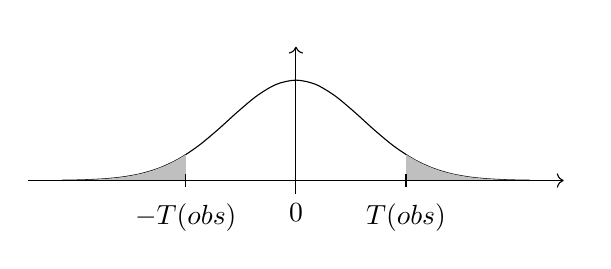
\begin{tikzpicture}[scale=0.85]
    % Draw the normal distribution curve
    \draw[domain=-3.5:3.5, smooth, variable=\x] plot ({\x}, {1.5*exp(-0.5*\x*\x)});

    % Shade the right tail area
    \fill[gray!50] (1.645,0) -- plot[domain=1.645:3.5, smooth, variable=\x] ({\x}, {1.5*exp(-0.5*\x*\x)}) -- (3.5,0) -- cycle;

    % Shade the left tail area
    \fill[gray!50] (-1.645,0) -- plot[domain=-1.645:-3.5, smooth, variable=\x] ({\x}, {1.5*exp(-0.5*\x*\x)}) -- (-3.5,0) -- cycle;

    % Label for the mean
    \node[below] at (0,-0.2) {$0$};

    % Label for the right critical value
    \node[below] at (1.645,-0.2) {$T(\text{obs})$};

    % Label for the left critical value
    \node[below] at (-1.645, -0.2) {$-T(\text{obs})$};

    % Axes
    \draw[->] (-4,0) -- (4,0) node[right] {};
    \draw[->] (0,-0.2) -- (0,2) node[above] {};

    \draw[-] (1.645,-0.1) -- (1.645,0.1) node[right] {};
    \draw[-] (-1.645,-0.1) -- (-1.645,0.1) node[right] {};


\end{tikzpicture}
\caption{
Density of standard normal $Z\sim \calN(0,1)$ random variable. Shaded area is equal to $p$-value $\Prob(|Z|\geq T(\text{obs}))$.
}\label{fig:normal_distr_two_sided}
\end{figure}




\end{center}

\begin{itemize}
  \item Two-sided test, using the half-normal distribution.
  \item Approximation valid for \(n \ge 30\); in practice \(n\) is usually much larger.
  \item Part of a family of tests based on random walks.
\end{itemize}
\end{frame}

\subsection{Two fundamental goodness-of-fit tests}
\begin{frame}{Two fundamental goodness-of-fit tests}
We use two general-purpose tests to assess the uniformity (and thus randomness) of PRNG output:
\begin{itemize}
  \item the \textbf{chi-square test}, and
  \item the \textbf{Kolmogorov–Smirnov (KS) test}.
\end{itemize}

\medskip
Example: three sets of $n=50$ numbers ($A$, $B$, $C$) are shown below.
The partition of $[0,1)$ is
\[
P_1=(0,0.15),\;
P_2=[0.15,0.35),\;
P_3=[0.35,0.6),\;
P_4=[0.6,0.8),\;
P_5=[0.8,1).
\]

\begin{center}
\includegraphics[width=0.8\linewidth]{figures_pdf/ch2_prng_sets_A_B_C_points_plot.pdf}
\end{center}

\begin{itemize}
  %\item Set $C$ originates from a quasirandom generator.
  \item Goal: determine whether sets $A$, $B$, and $C$ are consistent with uniform randomness.
\end{itemize}
\end{frame}

\subsection{Kolmogorov–Smirnov (KS) test}
% =======================
% Kolmogorov–Smirnov goodness-of-fit test
% =======================

\begin{frame}{Kolmogorov–Smirnov (KS) test}
We test whether $U_1,\ldots,U_n$ are distributed as $\calU[0,1)$.

Empirical c.d.f.:
\[
\hat{F}_n(t)=\frac{1}{n}\sum_{i=1}^n \ind(U_i\le t),
\qquad F(t)=t.
\]

Test statistic:
\[
D_n = \sup_{0\le t\le 1}|\hat{F}_n(t)-t|.
\]

If $U_i\sim\calU[0,1)$, then $\sqrt{n}D_n$ converges in distribution to
the \textsl{Kolmogorov distribution} $K(t)$:
\[
K(t)=\sum_{j=-\infty}^{\infty}(-1)^j e^{-2j^2t^2}.
\]
Critical values:
$\lambda_{0.1}=1.224$, $\lambda_{0.05}=1.358$, $\lambda_{0.01}=1.628$.
\end{frame}

\begin{frame}{Computation and $p$-value}
Order the sample: $U_{(1)}\le\cdots\le U_{(n)}$.

\[
D_n^+ = \max_i\!\left(\frac{i}{n}-U_{(i)}\right), \quad
D_n^- = \max_i\!\left(U_{(i)}-\frac{i-1}{n}\right),
\quad D_n=\max(D_n^+,D_n^-).
\]

$p$-value:
\[
p = 1 - K\!\left(\sqrt{n}D_n(\text{obs})
+ \frac{1}{6\sqrt{n}}
+ \frac{\sqrt{n}D_n(\text{obs})-1}{4n}\right).
\]
The correction improves small-$n$ accuracy
(see Vrbik, 1995).
\end{frame}

\begin{frame}{Example: sets $A$, $B$, $C$}
Empirical c.d.f.s for $A$, $B$, $C$
are compared with $F(t)=t$ for $\calU[0,1)$.

\[
D_n^A=0.1192,\quad D_n^B=0.2266,\quad D_n^C=0.0462.
\]
\[
p^A=44.17\%,\quad p^B=0.99\%,\quad p^C=99.97\%.
\]



\begin{center}
\begin{tabular}{ccc}
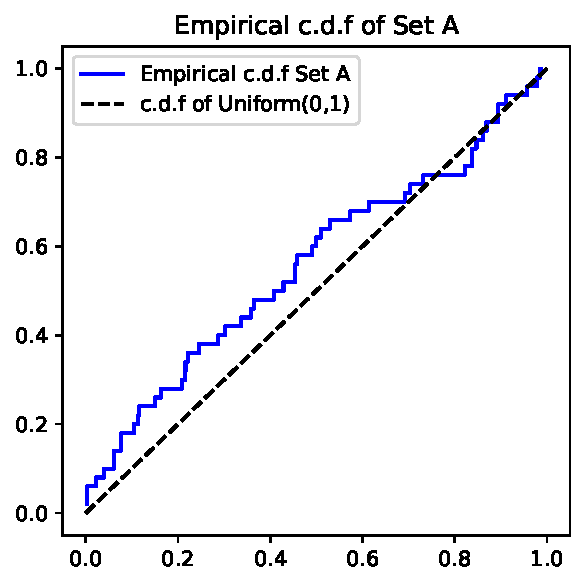
\includegraphics[width=0.25\linewidth]{figures_pdf/ch2_prng_sets_A_B_C_empCDF_of_setA.pdf}
&
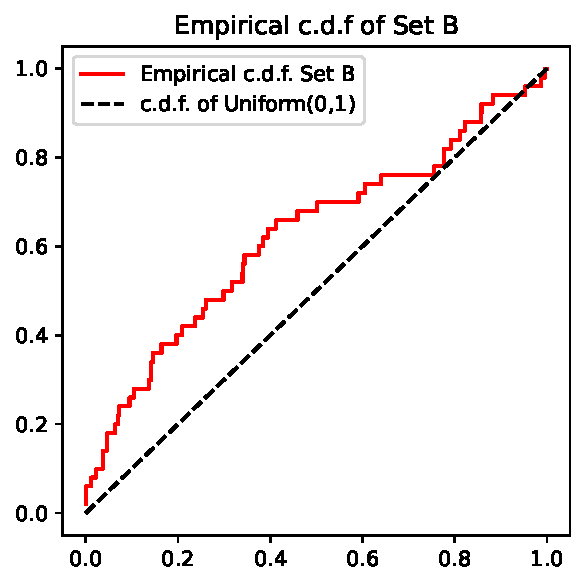
\includegraphics[width=0.25\linewidth]{figures_pdf/ch2_prng_sets_A_B_C_empCDF_of_setB.pdf} &
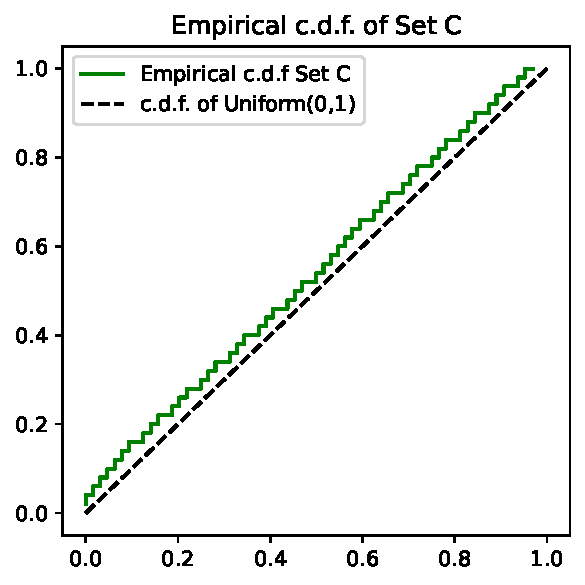
\includegraphics[width=0.25\linewidth]{figures_pdf/ch2_prng_sets_A_B_C_empCDF_of_setC.pdf}
\end{tabular}
\end{center}
\end{frame}

% =======================
% Chi-square goodness-of-fit
% =======================

\subsection{Chi-square goodness-of-fit (Pearson)}
\begin{frame}{Chi-square goodness-of-fit (Pearson)}
Multinomial setting: \(\mathrm{M}(r,p_1,\ldots,p_k)\).
Outcomes \(i=1,\ldots,k\) with probabilities \(p_i\); counts \(O_i\), expectations \(E_i=\Exp O_i=rp_i\).

\[
X_k^2=\sum_{i=1}^k \frac{(O_i-rp_i)^2}{rp_i}
      =\sum_{i=1}^k \frac{O_i^2}{rp_i}-r.
\]

As \(r\to\infty\): \(\;X_k^2 \convdistr \chi^2_{k-1}\).
For data: compute \(O_i\), then \(X_k^2\) and the \(p\)-value from \(\chi^2_{k-1}\).
\end{frame}

\begin{frame}{Using it for uniformity on \([0,1)\)}
Partition \( [0,1) \) into \(k\) bins \(P_i\) with lengths \(p_i=|P_i|\).
Given \(r\) samples, let \(O_i=\#\{u_j\in P_i\}\), then use
\[
X_k^2=\sum_{i=1}^k \frac{(O_i-rp_i)^2}{rp_i}, \qquad X_k^2 \approx \chi^2_{k-1}.
\]

\textbf{Rule of thumb:} each expected count \(\ge 5\):
\[
r \;\ge\; \left\lceil \frac{5}{\displaystyle \min_{1\le i\le k} p_i}\right\rceil.
\]

Notes:
\begin{itemize}
  \item Choice of \(k\), partition, and interpretation depends on application.
  \item For \(k\gg r\), prefer balls-and-boxes style tests.
\end{itemize}
\end{frame}

\begin{frame}{Example (sets \(A,B,C\); partition \(\calP\))}
Recall:
\begin{center}
\includegraphics[width=0.6\linewidth]{figures_pdf/ch2_prng_sets_A_B_C_points_plot.pdf}
\end{center}

With \(k=5\) bins from  , \(r=50\) satisfies the rule (\(p_{\min}=0.15\Rightarrow 34\)).

\[
X_A^2(\text{obs})=7.32,\quad
X_B^2(\text{obs})=16.25,\quad
X_C^2(\text{obs})=0.24,
\]
\[
p^A=11.99\%,\quad p^B=0.27\%,\quad p^C=99.35\% \quad (\chi^2_4).
\]

Interpretation:
\begin{itemize}
  \item \(A\): not rejected (consistent with uniformity).
  \item \(B\): rejected (very small \(p\)).
  \item \(C\): not rejected; very large \(p\) .
\end{itemize}

For large \(k\): \(\chi^2_k \eqdistr Z_1^2+\cdots+Z_k^2\), so
$
\frac{\chi^2_k - k}{\sqrt{2k}} \convdistr \mathcal{N}(0,1).
$
\end{frame}


\subsection{Statistical test contd.}

% =======================
% Spacing test — definition
% =======================

\begin{frame}{Spacing test}
Fix $(\alpha,\beta] \subset (0,1]$, let $\delta=\beta-\alpha$.
Indices hitting the interval:
\[
\{i\ge1: U_i\in(\alpha,\beta]\}=\{S_1<S_2<\cdots\},\quad
C_1=S_1,\ C_j=S_j-S_{j-1}\ (j\ge2).
\]
Under $\calH_0$ ($U_i$ i.i.d.\ $\calU[0,1)$):
\[
\Prob(C=l)= (1-\delta)^{\,l-1}\,\delta,\qquad l=1,2,\ldots
\]
(geometric on $\{1,2,\ldots\}$, mean $1/\delta$, var $(1-\delta)/\delta^2$).

For a finite sample $U_1,\ldots,U_n$:
\[
\{i\le n: U_i\in(\alpha,\beta]\}=\{S_1<\cdots<S_K\},\quad
C_1=S_1,\ldots, C_K=S_K-S_{K-1}.
\]
Choose bins
\[
A_0=\{0\},\,A_1=\{1\},\ldots,A_{s-1}=\{s-1\},\ A_s=\{s,s+1,\ldots\},
\]
with
\[
s\ \ge\ \max\!\left\{5,\ \left\lceil \frac{5(1-\delta)}{\delta}\right\rceil\right\}.
\]
\end{frame}

% =======================
% Spacing test — chi-square
% =======================

\begin{frame}{Spacing test: chi-square implementation}
Expected bin probabilities:
\[
p_i=\delta(1-\delta)^i\ (i=0,\ldots,s-1),\qquad
p_s=1-\sum_{i=0}^{s-1}p_i.
\]
Observed counts:
\[
O_i=\#\{j: C_j\in A_i\},\quad i=0,\ldots,s,\qquad \text{total }K.
\]
Test statistic:
\[
X^2(\text{obs})=\sum_{i=0}^{s}\frac{(O_i-Kp_i)^2}{Kp_i}\ \approx\ \chi^2_s\quad(\calH_0).
\]
Notes:
\begin{itemize}
  \item Sensitivity to bin choice—coarse vs.\ fine \(A_i\) may reveal/hide structure.
  \item Rule of thumb: ensure all \(Kp_i\gtrsim 5\).
\end{itemize}
\end{frame}

% =======================
% Serial test (incl. frequency tests)
% =======================
\begin{frame}{Serial test \((m,L)\) and special cases}
Partition \([0,1)^m\): split each axis into \(L\) equal parts; total \(k=L^m\) boxes.
Group \(n=mr\) values into \(r\) vectors
\[
\bfu_j=(u_{(j-1)m+1},\ldots,u_{jm})\in[0,1)^m,\quad j=1,\ldots,r.
\]


\begin{figure}[h]
\begin{center}6
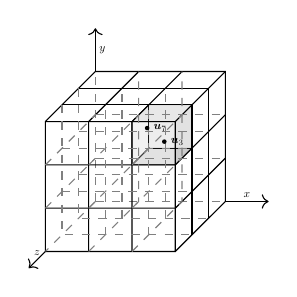
\begin{tikzpicture}[scale=0.55, every node/.style={scale=0.75}, transform shape]
  \draw[fill=gray!20, opacity=0.6] (3,3,3) -- (2,3,3) -- (2,2,3) -- (3,2,3); % przod
  \draw[fill=gray!45, opacity=0.6] (3,3,3) -- (2,3,3) -- (2,3,2) -- (3,3,2); % gora
  \draw[fill=gray!60, opacity=0.9] (3,3,3) -- (3,3,2) -- (3,2,2) -- (3,2,3); % prawy bok
  \draw[fill=gray!30, opacity=0.6] (3,2,3) -- (2,2,3) -- (2,2,2) -- (3,2,2); % dol
  \draw[fill=gray!10, opacity=0.5] (2,3,3) -- (2,3,2) -- (2,2,2) -- (2,2,3); % lewy  bok
  \draw[fill=gray!15, opacity=0.8] (3,3,2) -- (2,3,2) -- (2,2,2) -- (3,2,2); % przod



  \draw (3,0,0) coordinate (x) |- (0,3,0) coordinate [midway] (h) coordinate (y) -- (0,3,3) coordinate (a) -- (0,0,3) coordinate (z) -- (3,0,3) edge (x) -- (3,3,3) coordinate (v) edge (h)
  -- (a)  ;

  \draw [dashed, color=gray] (0,0,0) coordinate (o) edge (x) edge (y) -- (z);

  %\draw[->,color=red] (x) -- (o);


  \draw (1,0,3) -- (1,3,3) -- (1,3,0);
  \draw (2,0,3) -- (2,3,3) -- (2,3,0);

  \draw (0,3,1) -- (3,3,1) -- (3,0,1);
  \draw (0,3,2) -- (3,3,2) -- (3,0,2);


  \draw (0,1,3) -- (3,1,3) -- (3,1,0);
  \draw (0,2,3) -- (3,2,3) -- (3,2,0);


  \draw [dashed, color=gray] (1,0,1) -- (1,3,1) ;
  \draw [dashed, color=gray] (1,0,2) -- (1,3,2) ;

  \draw [dashed, color=gray] (2,0,1) -- (2,3,1);
  \draw [dashed, color=gray] (2,0,2) -- (2,3,2) ;

  \draw [dashed, color=gray] (0,3,1) -- (0,0,1) -- (3,0,1);
  \draw [dashed, color=gray] (0,3,2) -- (0,0,2) -- (3,0,2);

  \draw [dashed, color=gray] (1,0,3) -- (1,0,0) -- (1,3,0);
  \draw [dashed, color=gray] (2,0,3) -- (2,0,0) -- (2,3,0);

  \draw [dashed, color=gray] (0,1,0) -- (3,1,0);
  \draw [dashed, color=gray] (0,1,1) -- (3,1,1);
  \draw [dashed, color=gray] (0,1,2) -- (3,1,2);

  \draw [dashed, color=gray] (0,2,0) -- (3,2,0);
  \draw [dashed, color=gray] (0,2,1) -- (3,2,1);
  \draw [dashed, color=gray] (0,2,2) -- (3,2,2);

  \draw [dashed, color=gray] (1,1,3) -- (1,1,0);
  \draw [dashed, color=gray] (2,1,3) -- (2,1,0);

  \draw [dashed, color=gray] (1,2,3) -- (1,2,0);
  \draw [dashed, color=gray] (2,2,3) -- (2,2,0);

  \draw [dashed, color=gray] (0,1,3) -- (0,1,0) ;
  \draw [dashed, color=gray] (0,2,3) -- (0,2,0) ;

  \node [circle, minimum size=4pt, inner sep=0pt, fill, label=0:$\bfu_3$] at (2.4, 2.19, 2.1) {};
  \node [circle, minimum size=4pt, inner sep=0pt, fill, label=0:$\bfu_7$] at (2.1, 2.6, 2.35) {};
  \draw [->] (x) -- +(1pt,0,0) node [midway,above] {$x$};
  \draw [->] (y) -- +(0,1pt,0) node [midway,right] {$y$};
  \draw [->] (z) -- +(0,0,1pt) node [midway,above] {$z$};
  %\draw [color=brown] (v) -- ++(0,0,-1) coordinate (d) -- ++(-1,0,0) coordinate (e) -- ++(0,0,1) |- ++(1,-1,0) coordinate [midway] (f) -- ++(0,0,-1) coordinate (g) -- (d);
  %\draw [dashed] (e) -- ++(0,-1,0) coordinate (c) edge (f) -- (g);
  %\node [label=45:C] at (c) {};
 \end{tikzpicture}
\caption{Sample cube $[0,1)^m, m=3$, each side split into $L=3$ segments obtaining $k=L^3=27$
smaller sub-hypercubes. Sample points  $\bfu_3=(0.8, 0.73, 0.7)$ and $\bfu_7=(2.1, 2.6, 2.35)$ are presented together with the corresponding box
$A_{2,2,2}=\left\{(v_1,v_2,v_3): v_i\in\left({2\over 3},1\right), i=1,2,3\right\}$, or correspondingly $\bfy_3=\bfy_7=(2,2,2)$ and $A'_{2,2,2}=(2,2,2)$ (see description in the text).}
\label{fig:cube_bins}
\end{center}
\end{figure}
\end{frame}

\begin{frame}{Serial test \((m,L)\) and special cases}
The sub-hypercubes:
\begin{equation}\label{eq:sub-hypercubes}
A_{q_1,\ldots,q_m}=\left\{(v_1,\ldots,v_m): v_i \in \left[\frac{q_i}{L},\frac{q_i+1}{L}\right), \, i=1,\ldots,m\right\},
\end{equation}
where \(q_i \in \{0,\ldots,L-1\}\).
 Count the vectors:
\[
O_{q_1,\ldots,q_m} = \#\{i : \bfu_i \in A_{q_1,\ldots,q_m}\}, \quad (q_1,\ldots,q_m) \in \{0,\ldots,L-1\}^m.
\]
With \(k = L^m\), compute the chi-square statistic:
\[
X^2(\text{obs}) = \sum_{(q_1,\ldots,q_m) \in \{0,\ldots,L-1\}^m} \frac{(O_{q_1,\ldots,q_m} - r/k)^2}{r/k}.
\]
 Under the null hypothesis \(\calH_0\) (that the sequence is sampled from \(\calU[0,1)\)), for large \(r\), \(X^2\) is approximately chi-square distributed with \(k-1\) degrees of freedom.
\end{frame}

\begin{frame}{Serial test \((m,L)\) and special cases}
Partition \([0,1)^m\): split each axis into \(L\) equal parts; total \(k=L^m\) boxes.
Group \(n=mr\) values into \(r\) vectors
\[
\bfu_j=(u_{(j-1)m+1},\ldots,u_{jm})\in[0,1)^m,\quad j=1,\ldots,r.
\]
Counts per box \(O_{q_1,\ldots,q_m}\) with expected \(r/k\).
\[
X^2(\text{obs})=\sum_{(q_1,\ldots,q_m)}\frac{(O_{q_1,\ldots,q_m}-r/k)^2}{r/k}\ \approx\ \chi^2_{k-1}.
\]
Guidelines (Holst; L’Ecuyer et al.):
\begin{itemize}
  \item Fixed \(k\), \(r\to\infty\): \(X^2\to\chi^2_{k-1}\).
  \item \(r,k\to\infty\), \(r/k\to\gamma\in(0,\infty)\): standardized \(X^2\Rightarrow\calN(0,1)\);
        prefer \(0<\gamma<5\); for \(\gamma\ge5\) the \(\chi^2\) approx.\ improves.
\end{itemize}
Special cases:
\begin{itemize}
  \item \(m=1\) (frequency test): \(k=L\), \(O_i=\#\{j:y_j=i\}\), \(X^2=\sum_{i=0}^{k-1}\frac{(O_i-n/k)^2}{n/k}\).
  \item \(m=2\) (frequency of pairs): \(k=L^2\), \(O_{s,t}=\#\{j:(y_{2j-1},y_{2j})=(s,t)\}\),
        \(X^2=\sum_{s,t}\frac{(O_{s,t}-r/k)^2}{r/k}\).
\end{itemize}
\end{frame}

% =======================
% Tests based on "balls and boxes" scheme
% =======================

\subsection{Tests based on ``balls and boxes'' schemes}

\begin{frame}{Balls and boxes: setup}
We place \(r\) balls into \(k\) boxes, independently, with \(\Prob(\text{box }i)=p_i=1/k\) under \(\calH_0\).
This scheme underlies multiple tests of uniformity/independence.



\begin{center}
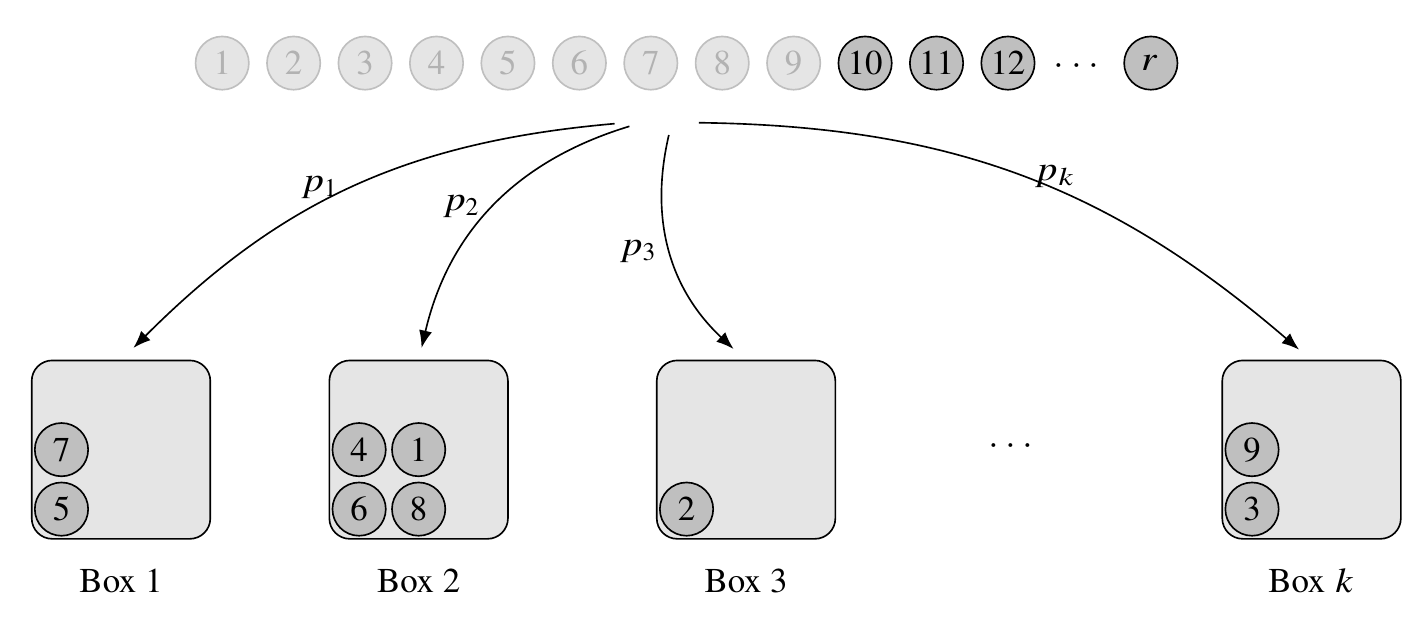
\includegraphics[width=0.8\linewidth]{pics/ball_into_boxes.png}
\end{center}
\end{frame}

% -----------------------

\begin{frame}{Birthday problem and collisions}
Birthday problem: \(k=365\) boxes (days), \(r\) balls (people).
\[
\Prob(\text{all unique})=\frac{(365)_r}{365^r},\qquad
p=1-\frac{(365)_r}{365^r}=1-\prod_{j=1}^{r-1}\Bigl(1-\frac{j}{365}\Bigr).
\]
General \(k\):
\[
p_{k,r}=1-\prod_{j=1}^{r-1}\Bigl(1-\frac{j}{k}\Bigr)\approx 1-\exp\!\left(-\frac{r^2}{2k}\right).
\]


\end{frame}

% -----------------------

\begin{frame}{Collision test (definition and approximation)}
Define the \textbf{number of collisions} \(C_{k,r}\): times a ball hits an already occupied box.
Then \(p_{k,r}=\Prob(C_{k,r}>0)\).
Given \(r\) balls, \(k\) boxes, the exact distribution of \(C_{k,r}\) is
\[
\Prob(C_{k,r}=c)=\frac{k(k-1)\cdots(k-r+c+1)}{k^r}\,S_2(r,r-c),\qquad c=0,1,\ldots,
\]
where \(S_2(\cdot,\cdot)\) are Stirling numbers of the second kind (counts of set partitions).

\medskip
\pause
Poisson approximation (no proof here): if \(r,k\to\infty\) with \(\tfrac{r^2}{2k}\to\lambda\in(0,\infty)\),
\[
\Prob(C_{k,r}=c)\ \to\ \frac{\lambda^c}{c!}e^{-\lambda},\qquad c=0,1,\ldots
\]
Mean comparison:
\[
\lambda\ \approx\ \frac{r^2}{2k},\qquad
\Exp C_{k,r}=r-k\Bigl(1-(1-\tfrac1k)^r\Bigr).
\]
Example: \(k=2^{20}, r=2^{14}\): \(r^2/(2k)=128\) vs.\ \(\Exp C_{k,r}=127.3282\).
\end{frame}

% -----------------------

\begin{frame}{Collision test in practice (binning \& chi-square)}
Convert a long PRNG stream into \(R\) experiments; each experiment yields one \(C_{k,r}\).
Group the values into bins with exact/approx.\ probabilities \((p_s)_{s=1}^B\), then apply
\[
X^2(\text{obs})=\sum_{s=1}^B \frac{(O_s-Rp_s)^2}{Rp_s}\ \approx\ \chi^2_{B-1}.
\]
\pause
Recommended parameters (bits): \(r=2^{14}\), \(k=2^{20}\) (e.g., \(m=20\)-bit “balls”), and use 10 bins as in Koçak.
Rule of thumb: ensure \(\min_s Rp_s\gtrsim 5\).
\end{frame}

% -----------------------

\begin{frame}{From sequences to balls and boxes}
Given \(u_1,\ldots,u_n\in[0,1)\), target \(m\)-dimensional structure and \(L\) bins/axis:
\[
y_i=\lfloor L u_i\rfloor,\qquad
\bfy_j=(y_{(j-1)m+1},\ldots,y_{jm}),\quad j=1,\ldots,r,\ n=mr.
\]
Boxes (sub-hypercubes) are indexed by \( (q_1,\ldots,q_m)\in\{0,\ldots,L-1\}^m\) (total \(k=L^m\)).
\begin{itemize}
  \item For collision test with bits: take \(m=20\) (or pairs to form base-4 symbols, \(m=10\)), so \(k=2^{20}\).
  \item For frequency/serial tests: use \(m=1\) (frequency) or \(m=2\) (frequency of pairs).
\end{itemize}
\end{frame}

% -----------------------


\begin{frame}{Poker test (5-tuples)}
Given $y_1,\ldots,y_n\in\bar{M}$ with $n=5r$, group into 5-tuples
\[
\bfy_j=(y_{5(j-1)+1},\ldots,y_{5j}),\quad j=1,\ldots,r.
\]
Following Knuth, each 5-tuple \( \bfy_i \) can be classified into one of the following simplified poker ranks:
\begin{description}
    \item \textbf{5 different}: all different,
    \item \textbf{4 different}: one pair,
    \item \textbf{3 different}: two pairs or three of a kind,
    \item \textbf{2 different}: full house or four of a kind,
    \item \textbf{1 different}: five of a kind.
\end{description}


\end{frame}




\begin{frame}{Poker test (5-tuples)}


Under $\calH_0$ ($Y_i\stackrel{i.i.d.}{\sim}\calU(\bar{M})$), with $S_2(5,s)$ the Stirling numbers of the second kind
\[
S_2(5,1)=1,\ S_2(5,2)=15,\ S_2(5,3)=25,\ S_2(5,4)=10,\ S_2(5,5)=1,
\]
the probability that a 5-tuple has exactly $s$ distinct values is
\[
p_s=\frac{(M)_s\,S_2(5,s)}{M^5},\qquad (M)_s=M(M-1)\cdots(M-s+1).
\]
\pause
Let $O_s=\#\{\text{5-tuples with }s\text{ distinct}\}$, $s=1,\ldots,5$. The chi-square statistic is
\[
X^2(\text{obs})=\sum_{s=1}^5\frac{(O_s-rp_s)^2}{rp_s}\ \approx\ \chi^2_{4}\quad(\calH_0).
\]

\smallskip
\textit{Notes:} Ensure all expected counts $rp_s\gtrsim 5$. In balls–boxes terms: $r$ balls into $k=5$ boxes (one box per “$s$ different” class).
\end{frame}



% =======================
% Tests based on random walks
% =======================

\subsection{Tests based on random walks}

\begin{frame}{Frequency (monobit) test}
Let bits $b_i\in\{0,1\}$ and define
\[
X_i = 2B_i - 1,\quad S_0=0,\quad S_k=\sum_{i=1}^k X_i.
\]
\pause
Under $\calH_0$, $S_n/\sqrt{n}\approx\calN(0,1)$ and
\[
T=|S_n|/\sqrt{n}\quad\text{has c.d.f. }G(z)=\Phi(z)-\Phi(-z)
      =\mathrm{erfc}\!\left(\frac{z}{\sqrt{2}}\right).
\]
Given $b_1,\ldots,b_n$:
\[
s_n=\sum_{j=1}^n(2b_j-1),\quad
T(\mathrm{obs})=\left|\frac{s_n}{\sqrt{n}}\right|,\quad
p=\mathrm{erfc}\!\left(\frac{T(\mathrm{obs})}{\sqrt{2}}\right).
\]
\vspace{-1ex}
This is equivalent to testing whether the walk deviates significantly from $0$.
\end{frame}

% -----------------------
%
% \begin{frame}{Frequency (monobit) test in blocks}
% Split $n=mr$ bits into $r$ blocks of length $m$.
% \[
% S_m^{(i)}=\sum_{j=1}^{m}(2B_{(i-1)m+j}-1),\quad
% Z_i=\frac{S_m^{(i)}}{\sqrt{m}},\quad i=1,\ldots,r.
% \]
% Under $\calH_0$: $Z_i\approx\calN(0,1)$ and
% \[
% \frac{1}{m}\sum_{i=1}^r(S_m^{(i)})^2
%  \eqdistr \sum_{i=1}^r Z_i^2 \sim \chi^2_r.
% \]
% Statistic:
% \[
% T(\mathrm{obs})=\frac{1}{m}\sum_{i=1}^r
%   \Bigl(\sum_{j=1}^{m}(2b_{(i-1)m+j}-1)\Bigr)^2,
% \]
% and the $p$-value is computed from $\chi^2_r$.
% \end{frame}

% -----------------------



\begin{frame}{Arcsine law test}
How does a ``typical'' realization of  $(S_k)$ look like?

\begin{figure}[h]
\centering
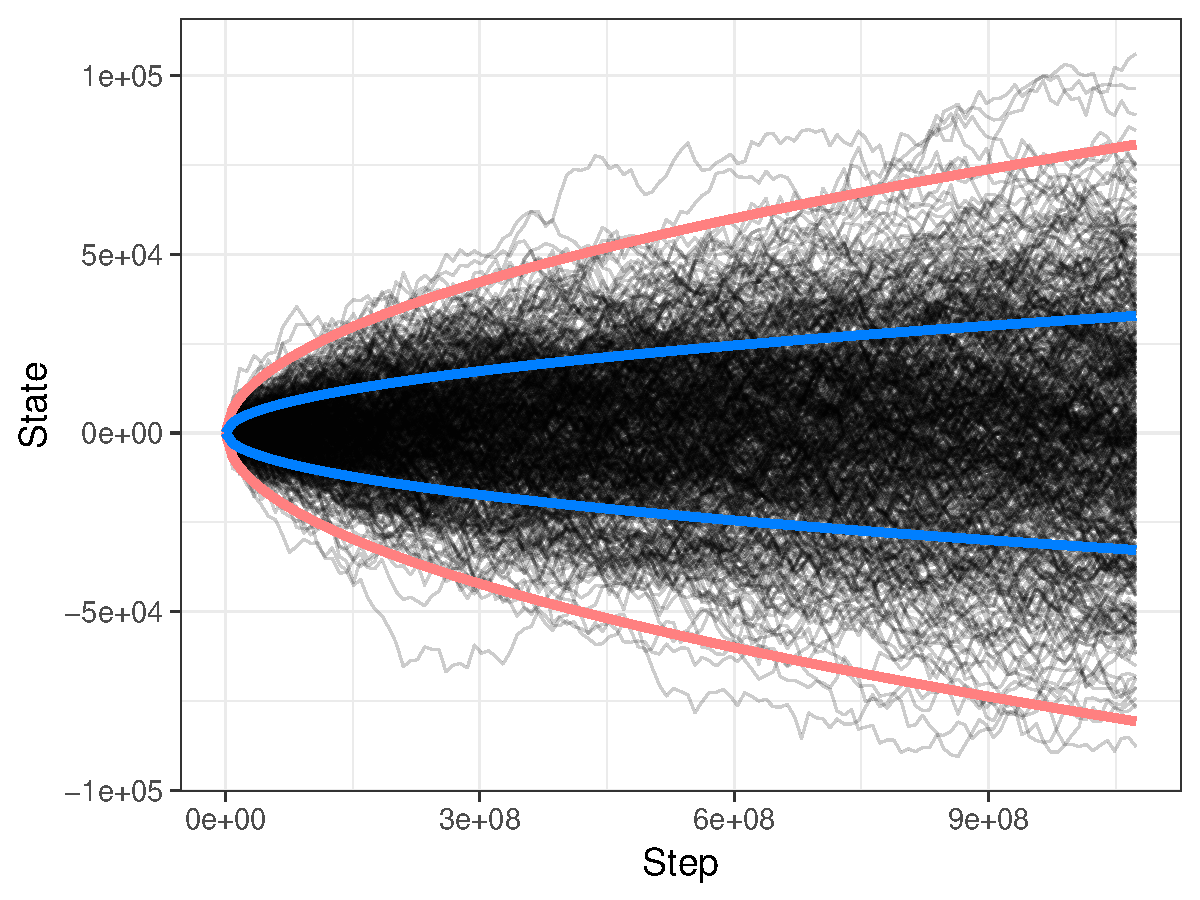
\includegraphics[scale=0.3]{figures/trajectories_6x8.pdf}
\caption{500 trajectories of random walks of length $n=2^{30}$.
\textcolor{blue}{Blue plot}: $\pm \sqrt{n}$, \textcolor{red}{red plot}: $\pm \sqrt{2n\log\log n}$.}\label{fig:500iter}
\end{figure}


\end{frame}



\begin{frame}{Arcsine law test}
For a random walk $(S_k)$ define
\[
D_k=\ind{(S_k>0 \vee S_{k-1}>0)},\quad
L^+_{2r}=\sum_{j=1}^{2r}D_j.
\]
I.e., $L^+_{2r}$ -- fraction of time random walk is above $x$-axis.
\medskip\par\noindent
\begin{center}
\begin{tabular}{lllll}
 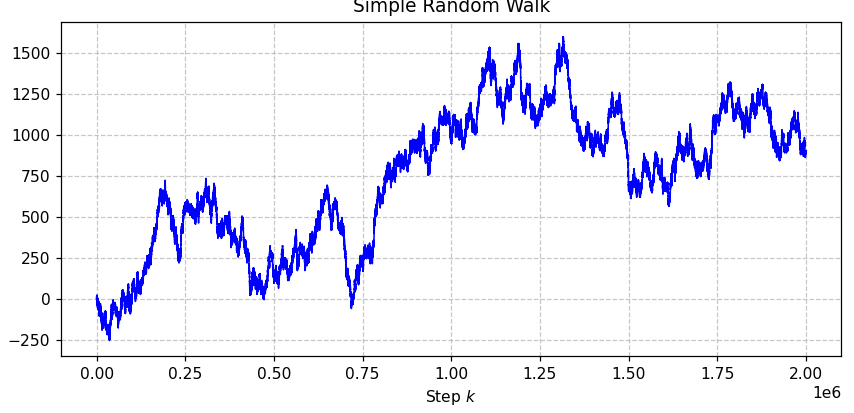
\includegraphics[scale=0.15]{pics/arcsine_walk1.png} &
  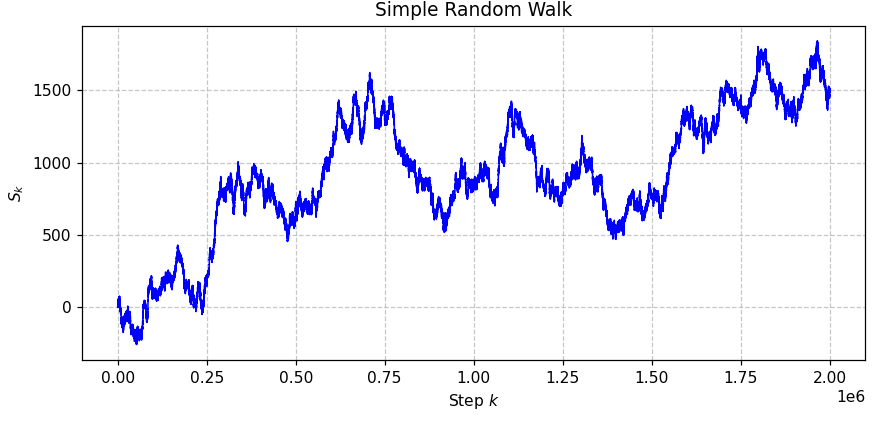
\includegraphics[scale=0.15]{pics/arcsine_walk2.png}\\
 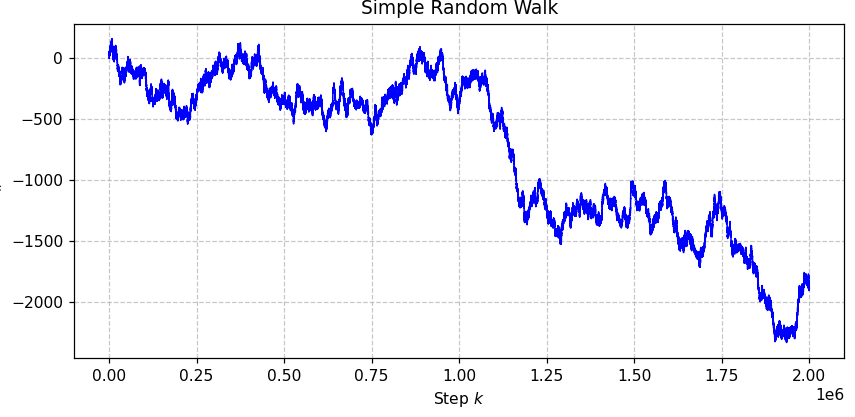
\includegraphics[scale=0.15]{pics/arcsine_walk3.png} &
  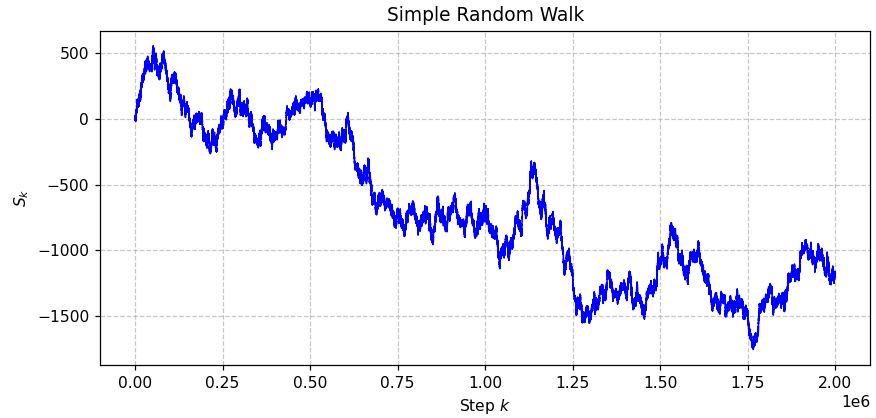
\includegraphics[scale=0.15]{pics/arcsine_walk4.png}\\
\end{tabular}
\end{center}


\end{frame}



\begin{frame}{Arcsine law test}
\begin{figure}[h]
 \centering
 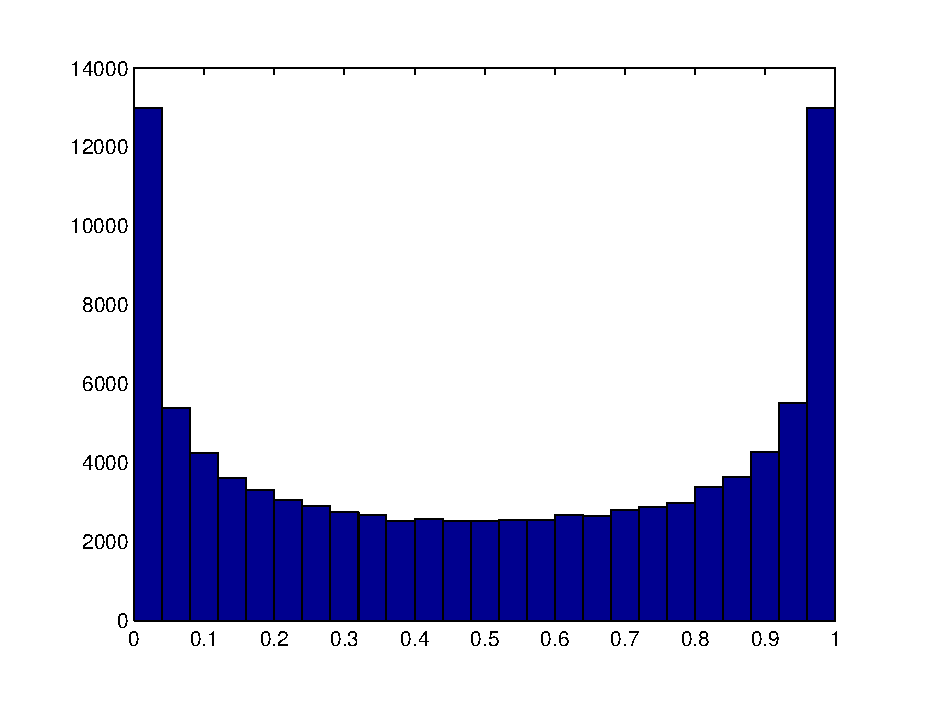
\includegraphics[height=6.3cm]{figures/arcsin.eps}
 \caption{Histogram for $L^{+}_{1000}; R=10^6$ replications, $25$ boxes.}
 \label{fig:arcsin}
\end{figure}

\end{frame}




\begin{frame}{Arcsine law test}
\[
D_k=\ind{(S_k>0 \vee S_{k-1}>0)},\quad
L^+_{2r}=\sum_{j=1}^{2r}D_j.
\]

\[
\mathrm{The\ arcsine\ law:}\qquad\qquad \Prob\!\left(\frac{L^+_{2r}}{2r}\le w\right)
 \to \frac{2}{\pi}\arcsin\sqrt{w}.
\]

\begin{figure}[h]
 \centering
 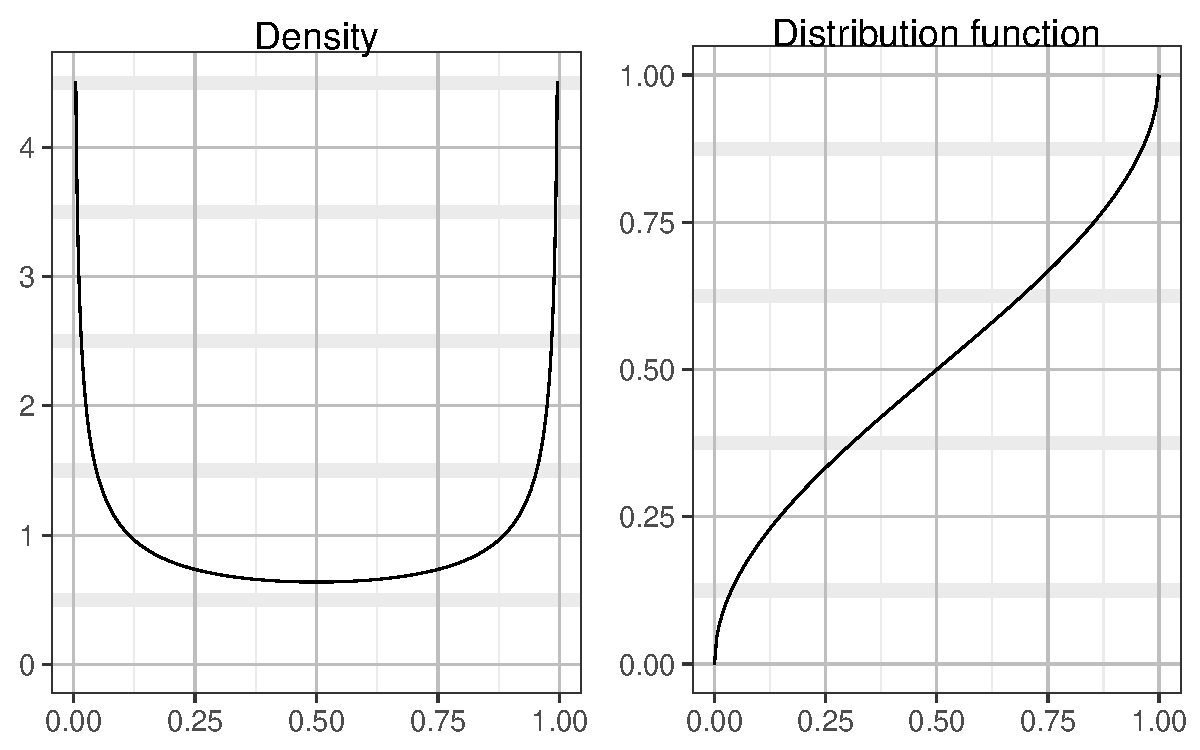
\includegraphics[height=4cm]{figures/arcsine_dist_5x8.pdf}
 \caption{Density function \(\frac{2}{\pi} \arcsin\sqrt{w}\) and the corresponding c.d.f.}
 \label{fig:arcsine_distr}
\end{figure}

\end{frame}









\begin{frame}{Arcsine law test}


Under $\calH_0$:
\[
p=\Prob(T_n>T(\mathrm{obs}))\approx
1-\frac{2}{\pi}\arcsin\sqrt{T(\mathrm{obs})}.
\]
Interpretation: a truly random walk spends most time either above or below zero, not equally on both sides.
\end{frame}

% =======================
% Permutation tests — derangements
% =======================

\subsection{Permutation tests}

\begin{frame}{Derangements: counting and asymptotics}
Let $\sigma$ be a random permutation of $[m]$ and $X=\#\{i:\sigma(i)=i\}$.
A derangement has $X=0$. Denote $\mathcal{D}_m$ the set of derangements, $d_m=|\mathcal{D}_m|$.

\textbf{Lemma.} \; $d_m=\displaystyle\sum_{k=0}^{m}(-1)^k{m\choose k}(m-k)!$.

\textit{Proof (inclusion–exclusion).}
Let $A_i=\{\sigma:\sigma(i)=i\}$. Then
\[
\Bigl|\bigcup_{i=1}^m A_i\Bigr|
= \pause \sum_{k=1}^{m}(-1)^{k+1}\!\!\!\sum_{1\le i_1<\cdots<i_k\le m}\!\!\!|A_{i_1}\cap\cdots\cap A_{i_k}|
= \pause \sum_{k=1}^{m}(-1)^{k+1}{m\choose k}(m-k)!.
\]
Thus $d_m=m!-\bigl|\cup_i A_i\bigr|=\sum_{k=0}^{m}(-1)^k{m\choose k}(m-k)!$. \qed

\end{frame}




\begin{frame}{Derangements: counting and asymptotics}
We have
$$d_m=m!-\bigl|\cup_i A_i\bigr|=\sum_{k=0}^{m}(-1)^k{m\choose k}(m-k)!
=m!\sum_{k=0}^{m}(-1)^k{1\over k!},$$
thus, the probability that a random permutation has no  fixed points
(i.e., probability of a derangements) is
\[
\frac{d_m}{m!}=\sum_{k=0}^{m}\frac{(-1)^k}{k!}\;\xrightarrow[m\to\infty]{}\;e^{-1},\qquad
\Bigl|e^{-1}-\sum_{k=0}^{m}\frac{(-1)^k}{k!}\Bigr|\le \frac{1}{(m+1)!}
\]


\end{frame}

% -----------------------

\begin{frame}{Derangement permutation test}
Input: $n=mr$ uniforms $u_1,\ldots,u_n$; group into $r$ $m$-tuples $\bfu_i$.
From $\bfu_i$ build $\sigma^{(i)}$ via \textsf{Fisher–Yates}.

Define the derangement indicator
\[
\xi_i=\begin{cases}
1,& \sigma^{(i)}\ \text{is a derangement},\\
0,& \text{otherwise}.
\end{cases}
\]
\pause
Under $\calH_0$: $\xi_i\stackrel{\text{i.i.d.}}{\sim}\mathrm{Bernoulli}(p_m)$ with
\[
p_m=\frac{d_m}{m!}=\sum_{k=0}^{m}\frac{(-1)^k}{k!}\approx e^{-1}.
\]
\pause
Test statistic (CLT/normal approx.):
\[
T(\mathrm{obs})=\frac{\bigl|\sum_{i=1}^{r}\xi_i-rp_m\bigr|}{\sqrt{r p_m(1-p_m)}},\qquad
p=\mathrm{erfc}\!\left(\frac{T(\mathrm{obs})}{\sqrt{2}}\right).
\]
\emph{Note:} For moderate $m$, use exact $p_m=d_m/m!$; for large $m$, $p_m\approx e^{-1}$.
\end{frame}

% -----------------------

\begin{frame}{Fixed–point permutation test (Poisson limit)}
Let $X=\#\{i:\sigma(i)=i\}$ for $\sigma\in\calS_m$. Exact distribution:
\[
\Prob(X=k)=\frac{1}{m!}{m\choose k}d_{m-k}.
\]
As $m\to\infty$, $d_{m-k}\sim (m-k)!e^{-1}$, hence
\[
\Prob(X=k)\ \to\ \frac{e^{-1}}{k!},\qquad X\ \Rightarrow\ \mathrm{Poisson}(1).
\]
\pause
\textbf{Test.} For each $\bfu_i$ form $\sigma^{(i)}$, then
\[
\xi_i=\#\{j:\sigma^{(i)}(j)=j\}\in\{0,1,2,\ldots\}.
\]
Bin counts (e.g.):
\[
A_0=\{0\},\ldots,A_9=\{9\},\quad A_{10}=\{10,11,\ldots\}.
\]
Let $O_j=\#\{i:\xi_i\in A_j\}$ and
\[
p_j=\begin{cases}
e^{-1}/j!, & j=0,\ldots,9,\\[2pt]
1-\sum_{k=0}^{9}e^{-1}/k!, & j=10.
\end{cases}
\]
Chi–square:
\[
X^2(\mathrm{obs})=\sum_{j=0}^{10}\frac{(O_j-rp_j)^2}{rp_j}\ \approx\ \chi^2_{10}\quad(\calH_0).
\]
(\emph{Rule of thumb:} ensure $rp_j\gtrsim5$; merge tail bins if needed.)
\end{frame}

\section{More on $p$-values}
\begin{frame}{Intuition behind $p$-values}
\begin{itemize}
 \item Suppose a PRNG produces $n$ bits. Under $\calH_0$, these are i.i.d.\ outcomes of fair coin flips.
 \item Each sequence of bits is equally likely, with probability $1/2^n$.
 \item For example, if $n=100$, observing all zeros has probability $7.88 \times 10^{-31}$.
 \item While possible, such an event is extremely unlikely --- we would reject the hypothesis of randomness.
\end{itemize}

\medskip
\noindent
For an event $E$ (e.g., ``at least 63 zeros among 100 bits''):
\[
\Prob(E)=\sum_{k=63}^{100}{100\choose k}\frac{1}{2^{100}}=0.00601.
\]
If we set $\alpha=0.01$, observing such an event leads to rejection of $\calH_0$.
\end{frame}

\begin{frame}{Formal definition and interpretation}
\begin{itemize}
 \item Test statistic $T$ summarizes the sequence under study.
 \item $\calH_0$: the sequence is i.i.d.\ and uniformly distributed.
 \item $\calH_1$: the sequence violates the randomness property.
 \item Two possible errors:
   \begin{itemize}
     \item Type I: reject $\calH_0$ when true.
     \item Type II: fail to reject $\calH_0$ when false.
   \end{itemize}
 \item The probability of Type I error is the significance level $\alpha$.
\end{itemize}

\medskip
For a right-tail test with continuous $F(t)$:
\[
p = 1 - F(T(\text{obs})).
\]
Larger $p$-values $\Rightarrow$ sequence behaves more randomly;
$p < \alpha$ $\Rightarrow$ reject $\calH_0$. \par
Most typically -- we compare PRNGs by $p$-values.
\end{frame}


\section{Second-level testing}

\begin{frame}{Second-level testing}

 So far, we performed \textbf{first-level testing}: we analyzed a single (usually long) sequence of numbers,
 computed one $p$-value, and decided whether to reject $\mathcal{H}_0$.
\pause
 Note: the statistic $T$ is computed for a random sequence, and therefore, the $p$-value   is itself \textbf{a random variable}.

 \pause
 Suppose $T$ is a continuous random variable with a strictly increasing cumulative distribution function (c.d.f.) $F$. For $t \in [0,1]$, we have:
\begin{align*}
\Prob(p \leq t) &= \Prob(1 - F(T) \leq t) = 1 - \Prob(F(T) \leq 1 - t) \\
&= 1 - \Prob\left( F^{-1}(F(T)) \leq F^{-1}(1 - t) \right) \\
&= 1 - \Prob\left( T \leq F^{-1}(1 - t) \right) = 1 - F\left( F^{-1}(1 - t) \right) = t.
\end{align*}
This implies that under the null hypothesis $\mathcal{H}_0$,
\textbf{the distribution of the $p$-value is uniform on $[0,1)$}.
Later we will prove:\medskip\par\noindent
\textbf{Lemma}:  If the test statistic has a continuous distribution under $\mathcal{H}_0$,
 then $p$-values are uniformly distributed $\calU[0,1)$


\end{frame}

\begin{frame}{Second-level testing: idea}


\medskip
\noindent
In \textbf{second-level testing}, instead of one long sequence, we:
\begin{itemize}
 \item[i)] Split the generator output into $R$ shorter subsequences;
 \item[ii)] Compute the statistic $T^{(i)}$ and $p$-value $p^{(i)}$ for each subsequence;
 \item[iii)] Test whether the $p$-values $p^{(1)}, \ldots, p^{(R)}$ are uniformly distributed on $[0,1)$.
\end{itemize}

\medskip
\noindent
Under $\calH_0$, the $p^{(i)}$ are i.i.d.\ $\calU[0,1)$ random variables.
The test checks this uniformity across all $R$ $p$-values.
\end{frame}






\begin{frame}{Chi-square uniformity test for $p$-values}
Let the generator output consist of $Rn$ numbers divided into $R$ subsequences of length $n$ each.
For each subsequence, compute $p^{(i)}$, $i=1,\ldots,R$.

\medskip

 \begin{figure}[h]
$$
\begin{array}{ccccc}
Rn \textrm{ numbers:} \\[2pt]
 u_1, u_2,\ldots, u_{Rn} \\[2pt]
 \textrm{ Split into } R \ \textrm{sequences of length } n \textrm{:} \\[15pt]
 \underbrace{
 \underbrace{u^{(1)}_1, \ldots, u^{(1)}_{n}}_{\footnotesize \textstyle \textrm{statistic } T^{(1)} \atop \footnotesize \textstyle p^{(1)}\textrm{-value}}
 \quad
 \underbrace{u^{(2)}_1, \ldots, u^{(2)}_{n}}_{\footnotesize \textstyle \textrm{statistic } T^{(2)} \atop \footnotesize \textstyle p^{(2)}\textrm{-value}}
 \quad
 \ldots
 \quad
 \underbrace{u^{(R)}_1, \ldots, u^{(R)}_{n}}_{\footnotesize \textstyle \textrm{statistic } T^{(R)} \atop {\footnotesize \textstyle p^{(R)}\textrm{-value} \atop \ }}
 }_{  \ \atop { {\small\textstyle \chi^2 \quad  \footnotesize \textstyle\textrm{UNIFORMITY TEST:}} }} \\
 p_{\chi^2,\textrm{final}}
\end{array}
$$
\caption{Sketch of second-level testing for tests with continuous statistic $T$.}\label{fig:second_level_testing}
\end{figure}
\end{frame}




\begin{frame}{Chi-square uniformity test for $p$-values}

Partition $[0,1)$ into $s$ equal intervals:
$ \displaystyle
P_i = \left[\frac{i-1}{s}, \frac{i}{s}\right), \quad i=1,\ldots,s.$
Let
\[
O_i = \#\{j : p^{(j)} \in P_i\}, \qquad E_i = \frac{R}{s}.
\]
Then compute
\[
X^2_{\rm final}(\text{obs}) = \sum_{i=1}^{s} \frac{(O_i - E_i)^2}{E_i}.
\]
Under $\calH_0$, $X^2_{\rm final}$ approximately follows $\chi^2_{s-1}$,
and the final $p$-value is
\[
p_{\chi^2,\text{final}} = 1 - F_{\chi^2,s-1}(X^2_{\rm final}(\text{obs})).
\]
\medskip
\noindent
Recommended: $1000 \le R \le 10000$, $2^{20} \le n \le 2^{32}$.
NIST suggests $s=10$, $\alpha \in [1/1000, 1/100]$ for the final $p$-value.
\end{frame}




\begin{frame}{Remarks on reliability and usage}
\begin{itemize}
 \item Second-level testing is generally \textbf{more reliable} than first-level testing.
 \item Choice of $n$ and $R$ affects sensitivity and reliability.
 \item Particularly useful when single-sequence $p$-values appear \textsl{suspiciously large},
       as in main Example.
 \item Aggregating $p$-values across multiple sequences
      may reveal non-randomness not visible in first-level testing.
\end{itemize}
\end{frame}

\begin{frame}{Example: second-level testing (1/4)}
Recall example of PRNGs that generated the sets $A$, $B$, and $C$:
\begin{figure}[h]
\begin{center}
 %\includegraphics[width=390pt]{pics/chi2_ks_points.png}\\
 %\includegraphics[width=390pt]{book_code/chapter_2/results/ch2_prng_sets_A_B_C_points_plot.pdf}
 \includegraphics[width=335pt]{figures_pdf/ch2_prng_sets_A_B_C_points_plot.pdf}
\end{center}
\caption{Three sets of $n=50$ points from $[0,1)$: set $A$ (\textcolor{blue}{blue}), set $B$ (\textcolor{red}{red}), and set $C$ (\textcolor{green}{green}).  }
\label{fig:chi2_ks_points}
\end{figure}


\medskip
\noindent
Recall:
\begin{itemize}
 \item The KS test accepted sets $A$ and $C$ but rejected $B$.
 \item The chi-square test confirmed these results.
 \item For $C$, $p$-values $>99\%$ were ``too good'' --- suspiciously close to~1.
\end{itemize}

\end{frame}


\begin{frame}{Example: second-level testing (2/4)}

Now we apply \textbf{second-level testing}:
\begin{itemize}
 \item $R = 200$ sequences, each of length $n = 50$.
 \item For each, we compute $p^{A_i}_{\rm KS}$, $p^{B_i}_{\rm KS}$, $p^{C_i}_{\rm KS}$,
       and similarly for $\chi^2$ tests.
 \item The uniformity of these $p$-values is tested using the $\chi^2$ test with   partition
       $\calP^{10}$ i.e.,
       $$P_i = \left[\frac{i-1}{10}, \frac{i}{10} \right), \quad 1 \leq i \leq 10.$$
       Results:

\end{itemize}
\begin{figure}[h]
\centering
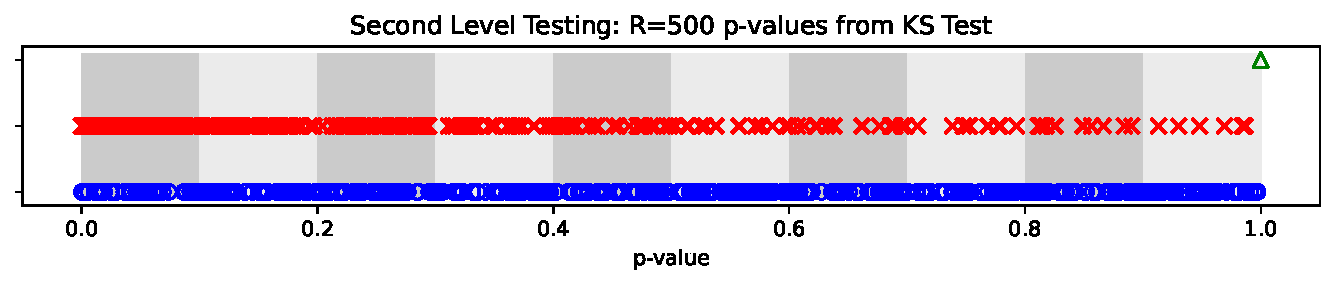
\includegraphics[width=0.85\textwidth]{figures_pdf/ch2_prng_sets_A_B_C_second_level_KS_pvalues.pdf}
\caption{$p$-values from the KS test:
$p^{A_i}_{\rm KS}$ (\textcolor{blue}{blue}),
$p^{B_i}_{\rm KS}$ (\textcolor{red}{red}),
$p^{C_i}_{\rm KS}$ (\textcolor{green}{green}),
for $i = 1,\ldots,R$.}
\label{fig:chi2_ks_p_values}
\end{figure}
\end{frame}




\begin{frame}{Example: second-level testing (3/4)}
The number of $p$-values within each interval $P_i$, $i=1,\ldots,10$, is shown below.

\begin{table}[h]
\centering
\small
\begin{tabular}{|l|l|c|c|c|c|c|c|c|c|c|c|}
\hline
   &   & $P_1$ & $P_2$ & $P_3$ & $P_4$ & $P_5$ & $P_6$ & $P_7$ & $P_8$ & $P_9$ & $P_{10}$ \\ \hline
\multirow{3}{*}{Chi-square test}
& $A$ & 57 & 51 & 52 & 52 & 52 & 38 & 57 & 38 & 55 & 48 \\
& $B$ & 189 & 79 & 57 & 45 & 41 & 18 & 29 & 27 & 9 & 6 \\
& $C$ & 0 & 0 & 0 & 0 & 0 & 0 & 0 & 0 & 0 & 500 \\ \hline
\multirow{3}{*}{KS-test}
& $A$ & 44 & 48 & 50 & 51 & 54 & 53 & 39 & 51 & 58 & 52 \\
& $B$ & 261 & 78 & 53 & 28 & 28 & 13 & 13 & 9 & 10 & 7  \\
& $C$ & 0 & 0 & 0 & 0 & 0 & 0 & 0 & 0 & 0 & 500 \\ \hline
\end{tabular}
\caption{Counts of $p$-values in intervals $P_i$ for partition $\calP^{10}$.
Under $\calH_0$ should be on average 50 in each one.}
\label{tab:sec-level-example-bins}
\end{table}
\pause
\begin{table}[h!]
\centering
\small
\begin{tabular}{|l|l|c|c|c|}
\hline
   &  &  {A} &  {B} &  {C} \\ \hline
\multirow{2}{*}{chi-square test}
& $\chi^2_{\rm final}(\mathrm{obs})$ & 8.56 & 518.56 & 4500.0 \\
& $p_{\rm final}$ & 0.479 & $6.09 \cdot 10^{-106}$ & 0.0 \\ \hline
\multirow{2}{*}{KS-test}
& $\chi^2_{\rm final}(\mathrm{obs})$ & 5.12 & 1083 & 4500.0 \\
& $p_{\rm final}$ & 0.824 & $2.16 \cdot 10^{-227}$ & 0.0 \\ \hline
\end{tabular}
\caption{Final $\chi^2$ and KS-test statistics and $p$-values for sets A, B, and C.}
\label{tab:comparison_tests}
\end{table}
\end{frame}



\begin{frame}{Example: second-level testing (4/4) -- generating sets $A$, $B$, and $C$}
We produce $R = 200$ sequences, each of length $n = 50$
(only one sequence per PRNG was shown earlier in Fig.~\ref{fig:chi2_ks_points}).
The procedure is as follows:
\begin{itemize}
 \item Generate $A_1,\ldots,A_R$ using Python's \texttt{NumPy} \texttt{PCG64} generator:\\
 \texttt{rng\_i = default\_rng(PCG64(seed=i))}, \quad
 \texttt{A\_i = rng\_i.random(size=n)}.
 \pause
 \item Obtain $B_1,\ldots,B_R$ by transforming $A_1,\ldots,A_R$:
 \[
 u_j^{B_i} = \frac{e^{u_j^{A_i}} - m_i}{M_i - m_i}, \quad
 m_i = \min_k(e^{u_k^{A_i}} - 1 - \varepsilon),\quad
 M_i = \max_k(e^{u_k^{A_i}} - 1 - \varepsilon),
 \]
 with $\varepsilon = 10^{-17}$.
 \pause
 \item Produce quasirandom sets $C_1,\ldots,C_R$ using
 \texttt{Halton} from \texttt{scipy.stats.qmc}, with \texttt{seed = i}.
\end{itemize}


\end{frame}




%
% \medskip
% \noindent
% \textbf{Conclusion:}
% \begin{itemize}
%  \item Sets $A$ behave as expected for a random source.
%  \item Sets $B$ are non-random (extremely small $p$-values).
%  \item Sets $C$ (quasirandom) yield ``too good'' results — $p_{\rm final} = 0$.
% \end{itemize}
% \end{frame}









\end{document}

